\documentclass[12pt,a4paper]{article}
\usepackage[T1]{fontenc}
\usepackage{natbib}
\usepackage{graphicx}
\usepackage{pdflscape}
\usepackage{amsmath}
\usepackage{multirow}
\renewcommand{\figurename}{Şekil}
\renewcommand{\refname}{Kaynakça}
\date{}
\usepackage{caption}
\captionsetup[table]{name=Tablo}

\title{TensorFlow ile Patates ve Mısır Yaprağı Hastalık Seti Üzerinde Eğitilmiş Bir Nesne Tanıma Modelinin C++'a Aktarılması ve Tespitin Gerçekleştirilmesi}
\author{Baranalp Öztürk}

\begin{document}
	\begin{figure}
		\centering
		
\includegraphics{ksbu.jpg}
	\end{figure}
	
	\maketitle
	
	\section{Giriş}
	\small
	\hspace{2em} Bu projede, Potato\_Late\_Blight, Potato\_Healthy, Potato\_Early\_Blight, Corn\_Healthy, Corn\_Gray\_Leaf\_Spot, Corn\_Common\_Rust, Corn\_Blight verileri toplanarak bir yapay zeka modeli geliştirildi. Python kullanılarak TensorFlow kütüphanesi ile bir derin öğrenme modeli oluşturuldu ve patates, mısır yaprak görüntüleri kullanılarak eğitildi. Model, farklı hastalıkları tanımak için optimize edildi, performansı değerlendirildi ve gerekli iyileştirmeler yapıldı. Eğitim tamamlandıktan sonra, model C++ programlama dili kullanılarak export edildi ve algılama işlemleri için entegre edildi. Bu, hastalık türlerini tanımlamak için bir görüntü işleme uygulaması oluşturulmasını sağladı. Uygulanan yöntem nesne tespit sürecini hızlandırdı.
	\newline \textbf{Anahtar Kelimeler:} Yapay zeka, Görüntü işleme, Derin öğrenme, TensorFlow, Hastalık tespiti
	
	
	\clearpage
				
		
		
		
			\section{Literatür Araştırması}			
				
		
		\hspace{3em} Mantarların Türk ve Dünya mutfaklarında kullanımı hızla artmakta, özellikle son
		yıllarda yabani mantar toplayıcılığı ve tüketiminde önemli artışlar yaşanmaktadır.
		Çevremizde sıkça gözlemlediğimiz gıda zehirlenmelerinin birçoğunu mantar zehirlenmeleri oluşturmaktadır. Öyle ki bu oran erişkinlerde mantar zehirlenmeleri tüm
		akut zehirlenme vakalarının yaklaşık yüzde 7'sini oluşturmaktadır. Ülkemizin kırsal kesimleri
		başta olmak üzere pek çok yerinde halk mantarları toplayarak gıda olarak tüketmektedir.
		Ülkemizde yeterli bilgiye sahip olmayan kişiler tarafından toplanan mantarların besin
		olarak tüketilmesi ile zehirlenmeler ve ne yazık ki ölümler görülebilmektedir. Bu
		çalışmada doğada kolaylıkla yetişebilen mantarların insanlar üzerindeki olumsuz
		etkilerini azaltmak amacıyla, insanların mantar kullanımında bilgi sahibi olmalarını
		sağlayarak bilinç düzeylerini artırmak için derin öğrenme tabanlı mobil uygulama
		tasarlanmıştır. Çalışmada ayrıca açık kaynak kod olarak sunulan, Google ve bağımsız
		geliştiriciler tarafından geliştirilen Tensorflow ve Keras kütüphaneleri kullanılmıştır.
		Android Studio ve Java programlama dili kullanılarak tasarlanan mobil uygulamaya derin
		öğrenme metotlarından VGG16 entegre edilerek kameradan görüntüsü alınan mantar
		tespit edilerek kullanıcıya özellikleri sunulmaktadır. Araştırma bulgularına uygulanan
		istatistiksel analizler sonucunda doğruluk oranı yüzde 81.75 olarak hesaplanmıştır
		\cite{akin2023dogada}.
		
		
		
		
		
		
		
		
		
		Meyve, Endonezya'da oldukça potansiyelli bir üründür. Hasat sırasında meyve üretimi oldukça bol olsa da, yavaş hasat süreci kaliteyi azaltır. Sonuç olarak, satış fiyatı düşüktür. Araştırmamızda, çoklu meyveleri sınıflandırmak için daha hızlı R-CNN kullanarak Derin Öğrenme yöntemi öneriyoruz. Kullanılan girişler mango ve pitaya meyveleridir. Veri kümesi, hasat zamanında bir çiftçiden alınan gerçek verilerden oluşur ve daha sonra eğitim nesne tespiti için mango ve pitaya olmak üzere 2 sınıfa ayrılır. TensorFlow platformunda MobileNet modelini kullandık. Bu çalışmada, yaklaşık yüzde 99'luk bir doğruluk skoru elde ettik. Bu yöntem, meyve kalitesini korumak için gerçek zamanlı olarak çoklu meyvelerin sıralama işlemini geliştirmek için oldukça uygundur \cite{8628566}.
		
		
		
		
		
		\clearpage
		
		
		Son yıllarda, nesne tespiti ve Desen Analizi alanında kapsamlı bir çalışma yapma konusunda büyük bir büyüme yaşanmaktadır. Sistemimizde, nesne tanıma ve desen analizi alanında makine öğrenimi ve derin öğrenme yaklaşımına dayalı bir tespit yöntemi üzerinde iyileştirmeler ve deneyler yaptık. Nesne tespitini, sınıf olasılıklarını ve sınırlayıcı kutuları mekansal olarak ayrılmış karşılık gelen bir gerileme sorunu olarak varsayıyoruz. Nesne tespiti, Desen Analizi ve izleme için birçok önde gelen algoritma tasarlanmıştır, bu da kenar izleme, renk bölütleme ve desen eşleştirmeyi içerir. Tek bir sinir ağı, bir döngüde tam görüntüden sınıf olasılıklarını ve sınırlayıcı kutuları doğrudan tahmin edebilir. Bu nedenle, Tensorflow'un yardımıyla video analizi yapmak için çeşitli sinir ağı algoritmalarını, YOLOv3, Tek Atışlı Çoklu tespit algoritmasını kullanıyoruz. Çerçeve, nesneleri sürekli olarak algılayacak ve kameradan algılanan girişlerden gerektiğinde kareler yakalayıp nesneyi tahmin etmek ve deseni eşleştirmek için kullanılabilir. Gerçek zamanlı video işleme ve tek bir kamera kullanılarak başarıyla tamamlanmıştır. Önerilen sistem, karmaşık, gerçek zamanlı, düz olmayan ortamlarda işlem yapabilecek esnek bir yapıya sahiptir\cite{9076486}.			
		\\*				
		Tabakalar ve dikkat mekanizmalarını derinleştirerek, küçük hedef kusurlarını tanıma yeteneğini artıran, arka plan gürültüsünü azaltan ve hesaplama verimliliğini artırmak için orijinal evrişim modüllerini derinlikli ayrılabilir evrişim ile değiştiren, hafif bir seramik karo tespit sistemi olan geliştirilmiş YOLOv5s modeline dayanan bir tespit yöntemi öneriyoruz. Deney sonuçları, modelimizin küçük kusurlar ve yetersiz özellik bilgisi ile ilgili sorunları etkili bir şekilde ele aldığını ve tespit doğruluğunu artırdığını göstermektedir					
		\cite{WAN202211085}.\pagebreak
		
\begin{figure}[h]
	\centering
	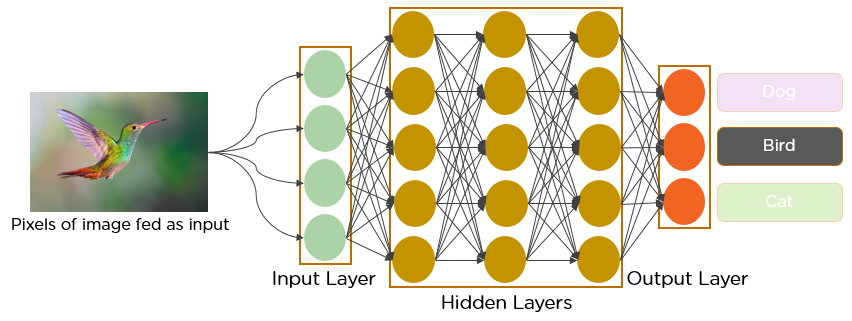
\includegraphics[width=\textwidth]{bird.png}
	\caption{CNN Model}
	\label{fig:grafik}
\end{figure}
		
\begin{figure}[h]
	\centering
	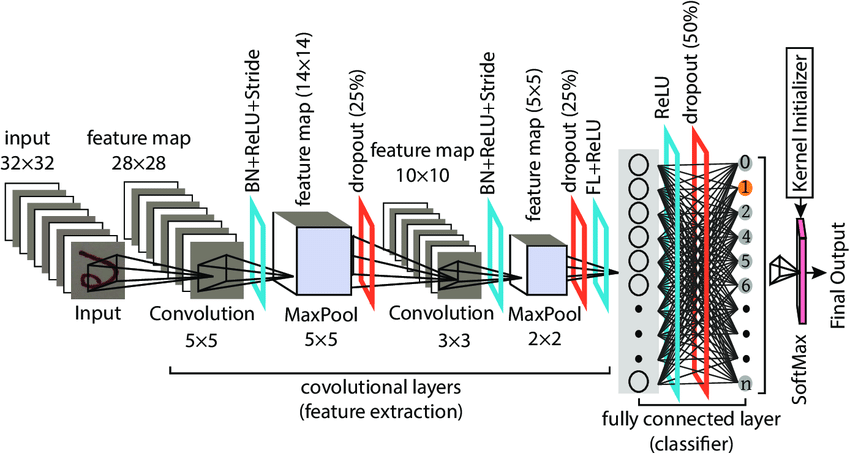
\includegraphics[width=\textwidth]{model.png}
	\caption{CNN Model}
	\label{fig:grafik}
\end{figure}

				
				
				
				
				
	
	
	\pagebreak
		\section{Metodoloji}
		\begin{enumerate}
			\item Modelin Export Edilmesi: Eğitilmiş TensorFlow modelinin C++ tarafında kullanılabilmesi için öncelikle modelin uygun bir formatta export edilmesi gerekir. TensorFlow, SavedModel veya FrozenGraph formatlarını destekler. Bu formatlardan birini seçerek modelinizi export etmelisiniz.
			\item TensorFlow C++ API'nin Kullanılması: TensorFlow C++ API, eğitilmiş modelin yüklenmesi ve görüntü işleme işlemlerinin gerçekleştirilmesi için kullanılır. API, modeli yüklemek, görüntü verilerini hazırlamak, tahmin yapmak ve sonuçları işlemek için gerekli olan fonksiyonları sağlar.
			\item 	Görüntü Verisinin Hazırlanması: Görüntü işleme işlemlerini gerçekleştirebilmek için girdi görüntülerin uygun formatta hazırlanması gerekir. Bu adımda, görüntülerin okunması, ön işleme adımlarının uygulanması ve TensorFlow tarafından kullanılabilen bir veri yapısına dönüştürülmesi gerekebilir.
			\item  Tahmin Yapma İşlemi: TensorFlow C++ API kullanılarak eğitilmiş model üzerinde tahmin yapılır. Girdi olarak hazırlanan görüntüler modelin girdisi olarak kullanılır ve modelden tahminler elde edilir.
			\begin{enumerate}
				\section*{TensorFlowlite C++ API Neleri İçerir}
				\item Graph Loading (Graf Yükleme): TensorFlow C++ API, eğitilmiş bir TensorFlow modelinin grafını (graph) yüklemek için fonksiyonlar sağlar. Bu, önceden eğitilmiş bir modelin mimarisini ve ağırlıklarını yüklemeyi mümkün kılar.
				\item Session Management (Oturum Yönetimi): API, TensorFlow modeliyle etkileşimde bulunmak için oturum (session) yönetimi sağlar. Bu, modelin belirli bir giriş verisine göre çıktıları tahmin etmek için oturum oluşturmayı ve sonlandırmayı içerir.
				\item Input Data Handling (Giriş Verisi İşleme): API, modelin giriş verilerini hazırlamak ve işlemek için gerekli fonksiyonları sağlar. Bu, giriş verilerini modelin beklediği formata dönüştürmeyi ve uygun şekilde işlemeyi içerir.
				\item Inference (Tahmin): API, yüklenen TensorFlow modelini kullanarak tahmin yapmak için fonksiyonlar sağlar. Bu, modelin giriş verisine dayalı olarak çıktıları tahmin etmeyi içerir.
		
				\pagebreak
				
					\section{Veriler}
				
				
				
				
		\hspace{3em} 	Bu çalışmada, toplamda 271 MB boyutunda farklı hastalık ve sağlık durumlarına sahip patates ve mısır yapraklarının resimlerini içeren bir veri kümesi kullanılmıştır. Bu veri kümesi ve resim sayıları şu şekildedir:
				
				\begin{itemize}
					\item Potato\_Late\_Blight: 1374 adet
					\item Potato\_Healthy: 826 adet
					\item Potato\_Early\_Blight: 2246 adet
					\item Corn\_Healthy: 2457 adet
					\item Corn\_Gray\_Leaf\_Spot: 732 adet
					\item Corn\_Common\_Rust: 2235 adet
					\item Corn\_Blight: 1560 adet
				\end{itemize}
				
				
				Her bir resim, 256x256 piksel boyutunda ve JPEG formatında kaydedilmiştir. Bu resimler, derin öğrenme modelinin eğitilmesi ve test edilmesi için kullanılmıştır. Bu veri kümesi, farklı hastalık ve sağlık durumlarının doğru bir şekilde tanınması ve sınıflandırılması için geliştirilen yapay zeka modellerinin eğitiminde kullanılan temel veri kaynağıdır.Bu projenin entegre edilmesi durumunda, yapay zeka destekli robotlarla yapılan tarım alanında önemli gelişmeler sağlanabilir. Yapay zeka ve görüntü işleme tekniklerinin kullanımıyla donatılan tarım robotları, tarım verimliliğini artırmak, iş gücünden tasarruf etmek ve tarım süreçlerini otomatikleştirmek için etkili bir araç olabilirler. Bu robotlar, çeşitli hastalık ve sağlık durumlarını tanımlayıp algılayarak, hastalık kontrolü ve yönetimi süreçlerini optimize edebilir, sağlıklı yaprakları tespit edebilir.
				
				 
				
				
				\clearpage
				

	\section{Bulgular}			
\
\begin{enumerate}
	\item Aşağıdaki tablolarda farklı model yapılandırmaları ve eğitim sonuçları verilmiş. Her bir modelde kullanılan katmanlar ve bu katmanların parametreleri farklılık gösteriyor. İncelediğimizde şu sonuçları çıkarabiliriz:
	
	\item Model Karmaşıklığı ve Performans İlişkisi: Model karmaşıklığı arttıkça (daha fazla katman ve parametre), eğitim kaybı ve doğrulama kaybı genellikle azalır. Ancak aynı zamanda aşırı uyum riski de artabilir, yani model eğitim verilerine aşırı uyum sağlayabilir ve genelleme yeteneği düşebilir.
	
	\item Dropout Katmanları: Dropout katmanları, özellikle daha derin modellerde kullanılarak aşırı uyumu azaltmaya yardımcı olur. Farklı modellerde dropout oranları değişkenlik gösteriyor (0.1, 0.2, 0.3 gibi).
	
	\item Tam Bağlantılı Katmanlar: Her modelde farklı sayıda tam bağlantılı katman bulunuyor (örneğin, 3 veya 4 adet). Bu katmanlar genellikle modelin çıkışına yakın yer alır ve sınıflandırma işlemini gerçekleştirir.
	
	\item Performans Metrikleri: Tüm modellerde eğitim doğruluğu ve doğrulama doğruluğu oldukça yüksek. Doğrulama kaybı da genellikle kabul edilebilir seviyelerde.
	
	\item Hiperparametreler: Farklı model yapılandırmalarında kullanılan hiperparametrelerin (örneğin, dropout oranları, filtre sayıları, kernel boyutları) etkisi belirgindir. Modelin performansı bu parametrelerin uygun bir şekilde seçilmesine bağlı olarak değişebilir.
	
	Sonuç olarak, en iyi modelin hangisi olduğunu belirlemek için belirli bir ölçüt (örneğin, doğrulama doğruluğu veya doğrulama kaybı) seçilmeli ve modeller bu ölçütlere göre karşılaştırılmalıdır. Tablolardaki verilere göre, en son tablodaki model (0.1167 kayıp, 0.9570 doğruluk) en düşük kayıp ve en yüksek doğruluğa sahip gibi görünmektedir.
		
\end{enumerate}

\begin{table}[htbp]
	\centering
	\caption{Model Katmanları ve Eğitim Sonuçları}
	\label{tab:model_layers}
	\resizebox{\textwidth}{!}{%
		\begin{tabular}{|c|l|}
			\hline
			\textbf{Katman Türü} & \textbf{Detaylar} \\
			\hline
			\multirow{2}{*}{Giriş Katmanı} & Conv2D(input\_shape=(256, 256, 1), filters=32, kernel\_size=(5, 5), activation="relu", padding="same") \\
			& MaxPooling2D(pool\_size=(2, 2)) \\
			\hline
			\multirow{2}{*}{Gizli Katman 1} & Conv2D(filters=16, kernel\_size=(3, 3), activation="relu", padding="same") \\
			& MaxPooling2D(pool\_size=(2, 2)) \\
			\hline
			\multirow{2}{*}{Gizli Katman 2} & Conv2D(filters=32, kernel\_size=(3, 3), activation="relu", padding="same") \\
			& MaxPooling2D(pool\_size=(2, 2)) \\
			\hline
			Gizli Katman 3 & Conv2D(filters=64, kernel\_size=(3, 3), activation="relu", padding="same") \\
			\hline
			Dropout Katmanı 1 & Dropout(0.2) \\
			\hline
			Düzleştirme Katmanı & Flatten() \\
			\hline
			\multirow{2}{*}{Tam Bağlantılı Katman 1} & Dense(units=128, activation="relu") \\
			& Dropout(0.2) \\
			\hline
			\multirow{2}{*}{Tam Bağlantılı Katman 2} & Dense(units=256, activation="relu") \\
			& Dropout(0.2) \\
			\hline
			Tam Bağlantılı Katman 3 & Dense(units=512, activation="relu") \\
			\hline
			\textbf{Eğitim Sonuçları} & \\
			\hline
			\multirow{2}{*}{\textbf{Kaybı}} & 0.1616 \\
			& (Doğrulama Kaybı: 0.3333) \\
			\hline
			\multirow{2}{*}{\textbf{Doğruluk}} & 0.9386 \\
			& (Doğrulama Doğruluğu: 0.9032) \\
			\hline
		\end{tabular}%
	}
\end{table}


\begin{table}[htbp]
	\centering
	\caption{Model Katmanları ve Eğitim Sonuçları}
	\label{tab:model_layers}
	\resizebox{\textwidth}{!}{%
		\begin{tabular}{|c|l|}
			\hline
			\textbf{Katman Türü} & \textbf{Detaylar} \\
			\hline
			\multirow{2}{*}{Giriş Katmanı} & Conv2D(input\_shape=(256, 256, 1), filters=32, kernel\_size=(5, 5), activation="relu", padding="same") \\
			& MaxPooling2D(pool\_size=(2, 2)) \\
			\hline
			\multirow{2}{*}{Gizli Katman 1} & Conv2D(filters=64, kernel\_size=(3, 3), activation="relu", padding="same") \\
			& MaxPooling2D(pool\_size=(2, 2)) \\
			\hline
			\multirow{2}{*}{Gizli Katman 2} & Conv2D(filters=128, kernel\_size=(3, 3), activation="relu", padding="same") \\
			& MaxPooling2D(pool\_size=(2, 2)) \\
			\hline
			\multirow{2}{*}{Gizli Katman 3} & Conv2D(filters=256, kernel\_size=(3, 3), activation="relu", padding="same") \\
			& MaxPooling2D(pool\_size=(2, 2)) \\
			\hline
			Dropout Katmanı & Dropout(0.1) \\
			\hline
			Düzleştirme Katmanı & Flatten() \\
			\hline
			\multirow{2}{*}{Tam Bağlantılı Katman 1} & Dense(units=128, activation="relu") \\
			& Dropout(0.1) \\
			\hline
			\multirow{2}{*}{Tam Bağlantılı Katman 2} & Dense(units=256, activation="relu") \\
			& Dropout(0.1) \\
			\hline
			Çıkış Katmanı & Dense(units=noOfClasses, activation="softmax") \\
			\hline
			\textbf{Eğitim Sonuçları} & \\
			\hline
			\multirow{2}{*}{\textbf{Kaybı}} & 0.1925 \\
			& (Doğrulama Kaybı: 0.2386) \\
			\hline
			\multirow{2}{*}{\textbf{Doğruluk}} & 0.9294 \\
			& (Doğrulama Doğruluğu: 0.9063) \\
			\hline
		\end{tabular}%
	}
\end{table}


\begin{table}[htbp]
	\centering
	\caption{Model Katmanları ve Eğitim Sonuçları}
	\label{tab:model_layers}
	\resizebox{\textwidth}{!}{%
		\begin{tabular}{|c|l|}
			\hline
			\textbf{Katman Türü} & \textbf{Detaylar} \\
			\hline
			\multirow{2}{*}{Giriş Katmanı} & Conv2D(input\_shape=(256, 256, 1), filters=32, kernel\_size=(5, 5), activation="relu", padding="same") \\
			& MaxPooling2D(pool\_size=(2, 2)) \\
			\hline
			\multirow{2}{*}{Gizli Katman 1} & Conv2D(filters=64, kernel\_size=(3, 3), activation="relu", padding="same") \\
			& MaxPooling2D(pool\_size=(2, 2)) \\
			\hline
			\multirow{2}{*}{Gizli Katman 2} & Conv2D(filters=128, kernel\_size=(3, 3), activation="relu", padding="same") \\
			& MaxPooling2D(pool\_size=(2, 2)) \\
			\hline
			\multirow{2}{*}{Gizli Katman 3} & Conv2D(filters=256, kernel\_size=(3, 3), activation="relu", padding="same") \\
			& MaxPooling2D(pool\_size=(2, 2)) \\
			\hline
			Dropout Katmanı & Dropout(0.3) \\
			\hline
			Düzleştirme Katmanı & Flatten() \\
			\hline
			\multirow{2}{*}{Tam Bağlantılı Katman 1} & Dense(units=128, activation="relu") \\
			& Dropout(0.3) \\
			\hline
			\multirow{2}{*}{Tam Bağlantılı Katman 2} & Dense(units=256, activation="relu") \\
			& Dropout(0.3) \\
			\hline
			\multirow{2}{*}{Tam Bağlantılı Katman 3} & Dense(units=512, activation="relu") \\
			& Dropout(0.3) \\
			\hline
			Tam Bağlantılı Katman 4 & Dense(units=1024, activation="relu") \\
			\hline
			Çıkış Katmanı & Dense(units=noOfClasses, activation="softmax") \\
			\hline
			\textbf{Eğitim Sonuçları} & \\
			\hline
			\multirow{2}{*}{\textbf{Kaybı}} & 0.1868 \\
			& (Doğrulama Kaybı: 0.3493) \\
			\hline
			\multirow{2}{*}{\textbf{Doğruluk}} & 0.9260 \\
			& (Doğrulama Doğruluğu: 0.8803) \\
			\hline
		\end{tabular}%
	}
\end{table}

\begin{table}[htbp]
	\centering
	\caption{Model Katmanları ve Eğitim Sonuçları}
	\label{tab:model_layers}
	\resizebox{\textwidth}{!}{%
		\begin{tabular}{|c|l|}
			\hline
			\textbf{Katman Türü} & \textbf{Detaylar} \\
			\hline
			\multirow{2}{*}{Giriş Katmanı} & Conv2D(input\_shape=(256, 256, 1), filters=32, kernel\_size=(5, 5), activation="relu", padding="same") \\
			& MaxPooling2D(pool\_size=(2, 2)) \\
			\hline
			\multirow{2}{*}{Gizli Katman 1} & Conv2D(filters=64, kernel\_size=(3, 3), activation="relu", padding="same") \\
			& MaxPooling2D(pool\_size=(2, 2)) \\
			\hline
			\multirow{2}{*}{Gizli Katman 2} & Conv2D(filters=128, kernel\_size=(3, 3), activation="relu", padding="same") \\
			& MaxPooling2D(pool\_size=(2, 2)) \\
			\hline
			\multirow{2}{*}{Gizli Katman 3} & Conv2D(filters=256, kernel\_size=(3, 3), activation="relu", padding="same") \\
			& MaxPooling2D(pool\_size=(2, 2)) \\
			\hline
			Dropout Katmanı & Dropout(0.3) \\
			\hline
			Düzleştirme Katmanı & Flatten() \\
			\hline
			\multirow{2}{*}{Tam Bağlantılı Katman 1} & Dense(units=128, activation="relu") \\
			& Dropout(0.3) \\
			\hline
			\multirow{2}{*}{Tam Bağlantılı Katman 2} & Dense(units=256, activation="relu") \\
			& Dropout(0.4) \\
			\hline
			\multirow{2}{*}{Tam Bağlantılı Katman 3} & Dense(units=512, activation="relu") \\
			& Dropout(0.5) \\
			\hline
			Tam Bağlantılı Katman 4 & Dense(units=1024, activation="relu") \\
			\hline
			Çıkış Katmanı & Dense(units=noOfClasses, activation="softmax") \\
			\hline
			\textbf{Eğitim Sonuçları} & \\
			\hline
			\multirow{2}{*}{\textbf{Kaybı}} & 0.2037 \\
			& (Doğrulama Kaybı: 0.2484) \\
			\hline
			\multirow{2}{*}{\textbf{Doğruluk}} & 0.9249 \\
			& (Doğrulama Doğruluğu: 0.9084) \\
			\hline
		\end{tabular}%
	}
\end{table}


\begin{table}[htbp]
	
	\caption{Model Katmanları ve Eğitim Sonuçları}
	\label{tab:model_layers}
	\resizebox{\textwidth}{!}{%
		\begin{tabular}{|c|l|}
			\hline
			\textbf{Katman Türü} & \textbf{Detaylar} \\
			\hline
			\multirow{2}{*}{Giriş Katmanı} & Conv2D(input\_shape=(256, 256, 1), filters=32, kernel\_size=(5, 5), activation="relu", padding="same") \\
			& MaxPooling2D(pool\_size=(2, 2)) \\
			\hline
			\multirow{2}{*}{Gizli Katman 1} & Conv2D(filters=32, kernel\_size=(3, 3), activation="relu", padding="same") \\
			& MaxPooling2D(pool\_size=(2, 2)) \\
			\hline
			\multirow{2}{*}{Gizli Katman 2} & Conv2D(filters=64, kernel\_size=(3, 3), activation="relu", padding="same") \\
			& MaxPooling2D(pool\_size=(2, 2)) \\
			\hline
			\multirow{2}{*}{Gizli Katman 3} & Conv2D(filters=128, kernel\_size=(3, 3), activation="relu", padding="same") \\
			& MaxPooling2D(pool\_size=(2, 2)) \\
			\hline
			Dropout Katmanı & Dropout(0.1) \\
			\hline
			Düzleştirme Katmanı & Flatten() \\
			\hline
			\multirow{2}{*}{Tam Bağlantılı Katman 1} & Dense(units=128, activation="relu") \\
			& Dropout(0.2) \\
			\hline
			\multirow{2}{*}{Tam Bağlantılı Katman 2} & Dense(units=256, activation="relu") \\
			& Dropout(0.2) \\
			\hline
			Tam Bağlantılı Katman 3 & Dense(units=512, activation="relu") \\
			\hline
			Çıkış Katmanı & Dense(units=noOfClasses, activation="softmax") \\
			\hline
			\textbf{Eğitim Sonuçları} & \\
			\hline
			\multirow{2}{*}{\textbf{Kaybı}} & 0.1167 \\
			& (Doğrulama Kaybı: 0.2210) \\
			\hline
			\multirow{2}{*}{\textbf{Doğruluk}} & 0.9570 \\
			& (Doğrulama Doğruluğu: 0.9334) \\
			\hline
		\end{tabular}%
	}
\end{table}		
\begin{figure}[h]
	\centering
	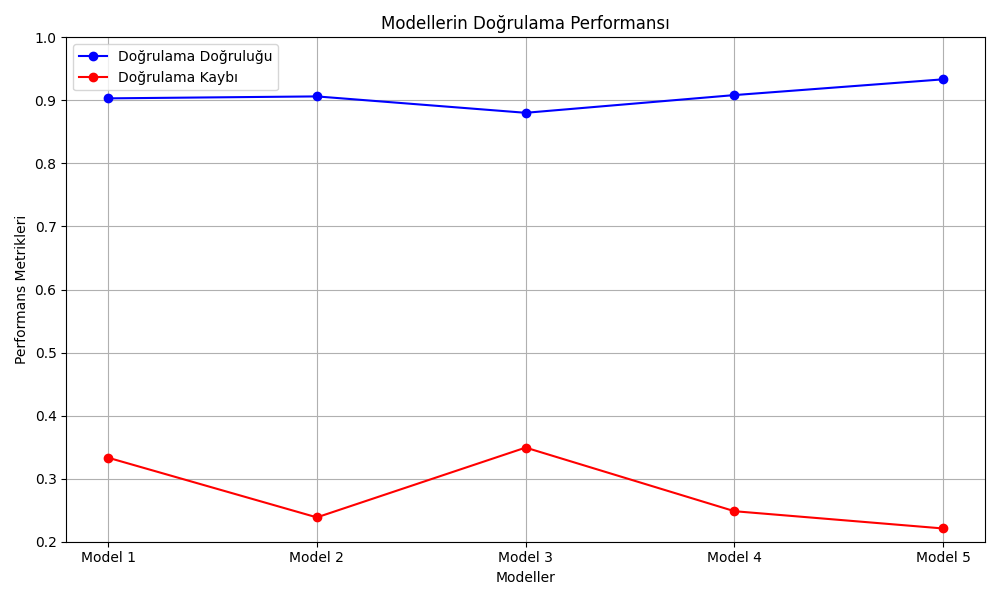
\includegraphics[width=\textwidth]{tablolar.png}
	\caption{Tabloların Değerlendirilmesi}
	\label{fig:grafik}
\end{figure}
\begin{figure}[h]
	\centering
	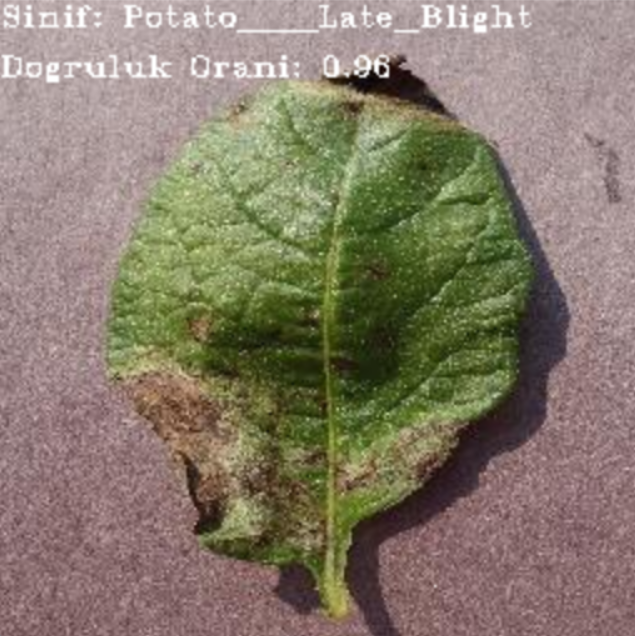
\includegraphics[width=\textwidth]{potato.png}
	\caption{Tespit Edilen Hastalık Örneği}
	\label{fig:grafik}
\end{figure}						
			\end{enumerate}
		\end{enumerate}


			
	
	\clearpage
			
			\section{Sonuçlar}	
		


	
	
	\hspace{2em} Sonuç olarak, TensorFlow modelini C++'a export edip çalıştırdığımızda, 130 resim üzerinde yapılan testlerde Python'a göre 2 saniye daha hızlı tespit ettiği sonucuna varıldı ve başarım oranlarının değişmediği gözlendi. Bu durum, endüstriyel alanlarda, özellikle toplu imalat yapan yerlerde (örneğin cam fabrikaları gibi) milisaniyelerin önemli olduğu durumlarda büyük bir avantaj sağlamaktadır. Nesne tespiti için Python'da eğitilen modelin C++'da TensorFlow ile nesne tespiti yapılmasının daha hızlı ve mantıklı olduğu sonucunu elde ettik. Bu yaklaşımı kullanarak, endüstriyel süreçlerde verimliliği artırmak ve tespit sürelerini azaltmak mümkündür.\newline


		
		
	
	

	\bibliographystyle{plain}
	\bibliography{references}
	
	
\end{document}